\documentclass[letterpaper,12pt]{article}
\usepackage{array}
\usepackage{threeparttable}
\usepackage{geometry}
\geometry{letterpaper,tmargin=1in,bmargin=1in,lmargin=1.25in,rmargin=1.25in}
\usepackage{fancyhdr,lastpage}
\pagestyle{fancy}
\lhead{}
\chead{}
\rhead{}
\lfoot{}
\cfoot{}
\rfoot{\footnotesize\textsl{Page \thepage\ of \pageref{LastPage}}}
\renewcommand\headrulewidth{0pt}
\renewcommand\footrulewidth{0pt}
\usepackage[format=hang,font=normalsize,labelfont=bf]{caption}
\usepackage{listings}
\lstset{frame=single,
  language=Python,
  showstringspaces=false,
  columns=flexible,
  basicstyle={\small\ttfamily},
  numbers=none,
  breaklines=true,
  breakatwhitespace=true
  tabsize=3
}
\usepackage{amsmath}
\usepackage{amssymb}
\usepackage{amsthm}
\usepackage{cite}
\usepackage{harvard}
\usepackage{setspace}
\usepackage{float,color}
\usepackage[pdftex]{graphicx}
\usepackage{hyperref}
\hypersetup{colorlinks,linkcolor=red,urlcolor=blue}
\theoremstyle{definition}
\newtheorem{theorem}{Theorem}
\newtheorem{acknowledgement}[theorem]{Acknowledgement}
\newtheorem{algorithm}[theorem]{Algorithm}
\newtheorem{axiom}[theorem]{Axiom}
\newtheorem{case}[theorem]{Case}
\newtheorem{claim}[theorem]{Claim}
\newtheorem{conclusion}[theorem]{Conclusion}
\newtheorem{condition}[theorem]{Condition}
\newtheorem{conjecture}[theorem]{Conjecture}
\newtheorem{corollary}[theorem]{Corollary}
\newtheorem{criterion}[theorem]{Criterion}
\newtheorem{definition}[theorem]{Definition}
\newtheorem{derivation}{Derivation} % Number derivations on their own
\newtheorem{example}[theorem]{Example}
\newtheorem{exercise}[theorem]{Exercise}
\newtheorem{lemma}[theorem]{Lemma}
\newtheorem{notation}[theorem]{Notation}
\newtheorem{problem}[theorem]{Problem}
\newtheorem{proposition}{Proposition} % Number propositions on their own
\newtheorem{remark}[theorem]{Remark}
\newtheorem{solution}[theorem]{Solution}
\newtheorem{summary}[theorem]{Summary}
%\numberwithin{equation}{section}
\bibliographystyle{aer}
\newcommand\ve{\varepsilon}
\newcommand\boldline{\arrayrulewidth{1pt}\hline}


\begin{document}

\begin{flushleft}
  \textbf{\large{Problem Set \#[1]}} \\
  MACS 30100, Dr. Evans \\
  Liqiang Yu
\end{flushleft}

\vspace{5mm}

\noindent\textbf{Problem 1}
Find a theoretical or statistical model from a recently published article (no earlier than 2013) in either the American Economic Review, American Journal of Political Science, or the American Journal of Sociology.

\textbf{Part (a).} 
I found a statistical model from a paper called ``How Do Hours Worked Vary with Income? Cross-Country Evidence and Implications." on American Economic Review 2018, 108(1). I am particularly interested in the relation between working hours and salary across or within countries.

\textbf{Part (b).} \textbf{Ref:} Bick, Alexander, Nicola Fuchs-Schündeln, and David Lagakos. 2018. "How Do Hours Worked Vary with Income? Cross-Country Evidence and Implications." American Economic Review, 108(1): 170-99.

\textbf{Part (c).} 
There are several linear regression models in this paper, corresponding to different subquestions. The one which I am especially interested in is the measurement of individual hours-wage elasticities (Figure \ref{FigEls}) by country. The regression model is 

\begin{equation*}
  \log(h_i)= \alpha + \beta_w \log(w_i)+\delta_1 age_i + \delta_2 age_{i}^2 + \epsilon_i.
\end{equation*}

\textbf{Part (d).} 
Types of variables are categorized below:
\begin{itemize}
\item Exogenous variables: $\log(h_i)$, $\log(w_i)$, $age_i$, $age_{i}^2$. 
\item Endogenous variables: $\alpha$, $\beta_w$, $\delta_1$, $\delta_2$, $\epsilon_i$.
\end{itemize}

  
\textbf{Part (e).} This is a linear, static and stochastic model. It is linear since it is a linear approach between a dependent variable and several independent variables. There is no time involving so it is static. Stochasticity comes from the error term $\epsilon_i$, which makes the model stochastic.

\textbf{Part (f).} A categorical variable indicating education level could have been introduced to this model, to evaluate individual hours-wage elasticities within groups with similar education level. 
\begin{figure}[htb]\centering\captionsetup{width=4.0in}
  \caption{\textbf{Elasticities for men across countries}}\label{FigEls}
  \fbox{\resizebox{2.5in}{1.6in}{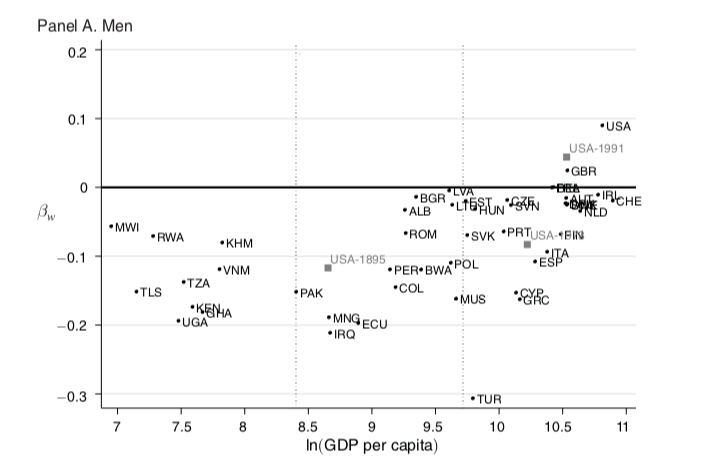
\includegraphics{elasticities.png}}}

\end{figure}

\newpage
\noindent\textbf{Problem 2}
Decision on getting married model.

\textbf{Part (a).} This is a prediction problem whose output set is \{0,1\}, so a logistic regression would be appropriate for this problem. To obtain the data, we can design a survey study which asks if the participant wants to get married or not and other demographic information. To obtain the model, there would be two steps. First, we want to use our training data to learn the parameters $\theta_i$:
\begin{gather*}
h_{\theta}(x)= g(\theta^Tx),\\
where\ y=0\ when\ h_{\theta}(x)<0.5\ and\ y=1\ for\ h_{\theta}(x)>0.5
\end{gather*}
Here, $g$ is the sigmoid function. After training, we then obtain the parameters $\theta$:
\begin{equation*}
  \theta^Tx= \theta_0 + \theta_1 x_1+ ... + \theta_n x_n.
\end{equation*}

For our interest, we want to focus on several exogenous variables:
\begin{equation*}
  \theta^Tx= \theta_0 + \theta_1 sex+ \theta_2 age + \theta_3 education\_level + \theta_4 income 
\end{equation*}

\textbf{Part (b).} The output set of the dependent endogenous variable is $y=1$ for getting married and $y=0$ for not getting married.

\textbf{Part (c).} This model satisfies a complete data generating process, that is, given all parameter $\theta_i$, we can obtain a binary classification by simulating data points for exogenous independent variables and putting them into our model.

\textbf{Part (d).} The possible key factors that may influence our outcomes are:
\begin{itemize}
\item Sex, Age, Education level, Income.
\end{itemize}

\textbf{Part (e).} I first came up with many factors by brainstorm, such as age, salary, family location, etc. Then I searched online articles or resorted to trustworthy data source to filter out valuable factors and lowly-correlated variables. 
\begin{itemize}
\item Sex: From the \href{https://www.thespruce.com/estimated-median-age-marriage-2303878}{Estimated Median Age of First Marriage by Gender}, we can observe a gap in age between men and women when first getting married.
\item Age: As above, the mean age of men for first marriage is 29.2 in 2015, so we anticipate men are prone to getting married when they are above a certain age.
\item Education level: ``College-educated adults are more likely to be married than less-educated adults.", \href{http://www.pewresearch.org/fact-tank/2015/12/04/education-and-marriage/}{Wendy Wang} says.
\item Income: ``marriage has sharply declined among people without college degrees, while staying steady among college graduates with higher incomes.", said by \href{https://www.nytimes.com/2017/09/25/upshot/how-did-marriage-become-a-mark-of-privilege.html}{Claire C. Miller}.
\end{itemize}

\textbf{Part (f).}
For practical significance, we can first use common knowledge to eliminate unreasonable factors and ``compute predicted/expected values for hypothetical cases" or calculate ``marginal effects", as mentioned in \href{https://arxiv.org/pdf/1301.1799.pdf}{How to calculate the practical significance of citation impact differences?}, to evaluate practical significance.

For statistical significance, since we are using logistic regression, we can calculate the p-value for each $\theta$ as well as looking at the R-square value. Besides, by modifying the number of features, we can compare between models and choose the significant one. Beyond manually select factors, we can apply a \href{http://www.medicine.mcgill.ca/epidemiology/Joseph/courses/EPIB-621/logselect.pdf}{Model Selection} on our model.


\end{document}

